\documentclass[10pt]{beamer}

\usetheme{metropolis}
\usepackage{appendixnumberbeamer}
\usepackage{booktabs}
\usepackage[scale=2]{ccicons}
\usepackage{pgfplots}
\usepackage{color}
\usepgfplotslibrary{dateplot}
\usepackage{xspace}
\newcommand{\themename}{\textbf{\textsc{metropolis}}\xspace}

\usepackage{stmaryrd}
\usepackage{amsmath}
\usepackage{verbatim}
\usepackage{tikz}
\usepackage{siunitx}
\usepackage{color}
\usepackage[normalem]{ulem}
\usetikzlibrary{calc,decorations.pathmorphing,patterns}
\usepackage{amssymb}
\usepackage{amsfonts}
\usepackage{amscd}
\usepackage{amsthm}
\usepackage{mathrsfs}
\usepackage{enumerate}
\usepackage{mathtools}
\usepackage{booktabs}
\usepackage{array}
\usepackage{nth}
\usepackage{lipsum}


%%%%%%%%%%%%%%%%%%%%%%%%%%%%%list %%%%%%%%%%%%%%%%%
\usepackage{textcomp}           % To use with matlab-prettifier
\usepackage{listings}
\usepackage[framed , numbered]{matlab-prettifier}
\usepackage{listings}
%%%%%%%%%%%%%%%%%end of list%%%%%%%%%%%%%%%%%%%%%

%%%%%%%%%%%%%%%%%%%%%%%%%%%%%%%%%%%%%%%%%%%%%%%%%%%%%%%%%%%%%%%%%%%%%%%%%
%%%% The following is for fancy box %%%%%%%%%%%%%%
\usepackage[framemethod=TikZ]{mdframed}
%%%%%%%%%%%%% Theorem %%%%%%%%%%%%
\newenvironment{thm}[2][]{%
\ifstrempty{#1}%
{\mdfsetup{%
frametitle={%
\tikz[baseline=(current bounding box.east),outer sep=0pt]
\node[anchor=east,rectangle,fill=red!20]
{\strut Theorem};}}
}%
{\mdfsetup{%
frametitle={%
\tikz[baseline=(current bounding box.east),outer sep=0pt]
\node[anchor=east,rectangle,fill=red!20]
{\strut Theorem #1};}}%
}%
\mdfsetup{innertopmargin=1pt,linecolor=red!20,%
linewidth=2pt,topline=true,%
frametitleaboveskip=\dimexpr-\ht\strutbox\relax
}
\begin{mdframed}[]\relax%
\label{#2}}{\end{mdframed}}
%%%%%%%%%%%%%%Lemma%%%%%%%%%%%%%%%%%%%%%%%%%%%%%%%%%%%%%%%%%%%%%%%%%%%%%%
\newcounter{lem}[section] \setcounter{lem}{0}
\renewcommand{\thelem}{}
\newenvironment{lem}[2][]{%
\refstepcounter{lem}%
\ifstrempty{#1}%
{\mdfsetup{%
frametitle={%
\tikz[baseline=(current bounding box.east),outer sep=0pt]
\node[anchor=east,rectangle,fill=green!20]
{\strut Lemma~\thelem};}}
}%
{\mdfsetup{%
frametitle={%
\tikz[baseline=(current bounding box.east),outer sep=0pt]
\node[anchor=east,rectangle,fill=green!20]
{\strut Lemma~\thelem:~#1};}}%
}%
\mdfsetup{innertopmargin=1pt,linecolor=green!20,%
linewidth=2pt,topline=true,%
frametitleaboveskip=\dimexpr-\ht\strutbox\relax
}
\begin{mdframed}[]\relax%
\label{#2}}{\end{mdframed}}
%%%%%%%%%%%%%%%%%%%%%%%%%%%%%%%%%%%%%%%%%%%%%%%%%%%%%%%%%%%%%%%%%%%%%%%
%Corollary
\newenvironment{cor}[2][]{%
\ifstrempty{#1}%
{\mdfsetup{%
frametitle={%
\tikz[baseline=(current bounding box.east),outer sep=0pt]
\node[anchor=east,rectangle,fill=blue!30]
{\strut Corollary};}}
}%
{\mdfsetup{%
frametitle={%
\tikz[baseline=(current bounding box.east),outer sep=0pt]
\node[anchor=east,rectangle,fill=blue!30]
{\strut Corollary:~#1};}}%
}%
\mdfsetup{innertopmargin=1pt,linecolor=blue!30,%
linewidth=2pt,topline=true,%
frametitleaboveskip=\dimexpr-\ht\strutbox\relax
}
\begin{mdframed}[]\relax%
\label{#2}}{\end{mdframed}}
%%%%%%%%%%%%%%%%%%%%%%%%%%%%%%%%%%%%%%%%%%%%%%%%%%%%%%%%%%%%%%%%%%%%%%%
%Proof
\newenvironment{prove}[2][]{%
\ifstrempty{#1}%
{\mdfsetup{%
frametitle={%
\tikz[baseline=(current bounding box.east),outer sep=0pt]
\node[anchor=east,rectangle,fill=red!20]
{\strut Proof};}}
}%
{\mdfsetup{%
frametitle={%
\tikz[baseline=(current bounding box.east),outer sep=0pt]
\node[anchor=east,rectangle,fill=red!20]
{\strut Proof:~#1};}}%
}%
\mdfsetup{innertopmargin=1pt,linecolor=red!20,%
linewidth=2pt,topline=true,%
frametitleaboveskip=\dimexpr-\ht\strutbox\relax
}
\begin{mdframed}[]\relax%
\label{#2}}{\end{mdframed}}
%%%%%%%%%%%%%%%%%%%%%%%%%%%%%%%%%%%%%%%%%%%%%%%%%%%%%%%%%%%%%%%%%%%%%%%
%Defintion
\newcounter{drf}[section]\setcounter{drf}{0}
\renewcommand{\thedrf}{}
\newenvironment{drf}[2][]{%
\refstepcounter{drf}%
\ifstrempty{#1}%
{\mdfsetup{%
frametitle={%
\tikz[baseline=(current bounding box.east),outer sep=0pt]
\node[anchor=east,rectangle,fill=orange!20]
{\strut Definition~\thedrf};}}
}%
{\mdfsetup{%
frametitle={%
\tikz[baseline=(current bounding box.east),outer sep=0pt]
\node[anchor=east,rectangle,fill=orange!20]
{\strut Definition~\thedrf:~#1};}}%
}%
\mdfsetup{innertopmargin=1pt,linecolor=orange!20,%
linewidth=2pt,topline=true,%
frametitleaboveskip=\dimexpr-\ht\strutbox\relax
}
\begin{mdframed}[]\relax%
\label{#2}}{\end{mdframed}}
%%%%%%%%%%%%%%%%%%%%%%%%%%%%%%%%%%%%%%%%%%%%%%%%%%%%%%%%%%%%%%%%%%%%%%%%%%%
% end of self defined label
%%%%%%%%%%%%%%%%%%%%%%%%%%%%%%%%%%%%%%%%%%%%%%%%%%%%%%%%%%%%%%%%%%%%%%%%%%%


%%%%%%%%%%%%%% For double curly bracket%%%%%%%%%%%%%%%%
\usepackage{xparse}

\NewDocumentCommand{\dgal}{sO{}m}{%
  \IfBooleanTF{#1}
    {\dgalext{#3}}
    {\dgalx[#2]{#3}}%
}

\NewDocumentCommand{\dgalext}{m}{%
  \sbox0{%
    \mathsurround=0pt % just for safety
    $\left\{\vphantom{#1}\right.\kern-\nulldelimiterspace$%
  }%
  \sbox2{\{}%
  \ifdim\ht0=\ht2
    \{\kern-.45\wd2 \{#1\}\kern-.45\wd2 \}%
  \else
    \left\{\kern-.5\wd0\left\{#1\right\}\kern-.5\wd0\right\}%
  \fi
}

\NewDocumentCommand{\dgalx}{om}{%
  \sbox0{\mathsurround=0pt$#1\{$}%
  \sbox2{\{}%
  \ifdim\ht0=\ht2
    \{\kern-.45\wd2 \{#2\}\kern-.45\wd2 \}%
  \else
    \mathopen{#1\{\kern-.5\wd0 #1\{}
    #2
    \mathclose{#1\}\kern-.5\wd0 #1\}}
  \fi
}
%%%%%%%%%%%%%%%%



%%%%%%%%%%%%%%%%%%%%%%%%%%%%%%%%%%%%%

\usepackage{animate}

\graphicspath{{./fig/}}


%%%%%%%%%%%%%% define color %%%%%%%%%%%%%%%%%%
\definecolor{DarkFern}{HTML}{407428}
\definecolor{DarkCharcoal}{HTML}{4D4944}
\colorlet{Fern}{DarkFern!85!white}
\colorlet{Charcoal}{DarkCharcoal!85!white}
\colorlet{LightCharcoal}{Charcoal!50!white}
\colorlet{AlertColor}{orange!80!black}
\colorlet{DarkRed}{red!70!black}
\colorlet{DarkBlue}{blue!70!black}
\colorlet{DarkGreen}{green!70!black}

\newcommand{\I}{\mathrm{i}}




%%%%%%%%%%%%%%%%%%%%%%%%%%%%%%%%%%%%%%
%\newcommand{\G}{\alert{G}}  % change color of main author



%%%%%%%%%%%%% Title Page %%%%%%%%%%%%%%%%%%%

\title{MAST90026 Computational Differential\\Equations: Week 7}
%\subtitle{A modern beamer theme}
\date{Semester 1 2024}
\author{Jesse Collis\\Modified from Hailong Guo (2022)}
\institute{The University of Melbourne}
\titlegraphic{\vspace{6cm}\flushright\includegraphics[height=2cm]{logo.png}}


\begin{document}

\maketitle


%
%
%\begin{frame}{Table of contents}
%  \setbeamertemplate{section in toc}[sections numbered]
%  \tableofcontents[hideallsubsections]
%\end{frame}


%-=-=-=-=-=-=-=-=-=-=-=-=-=-=-=-=-=-=-=-=-=-=-=-=
%
%	SECTION: 
%
%-=-=-=-=-=-=-=-=-=-=-=-=-=-=-=-=-=-=-=-=-=-=-=-=
%\section{Method of Weighted Residuals}








%-=-=-=-=-=-=-=-=-=-=-=-=-=-=-=-=-=-=-=-=-=-=-=-=
%	FRAME:
%-=-=-=-=-=-=-=-=-=-=-=-=-=-=-=-=-=-=-=-=-=-=-=-=
\begin{frame}{Sparse solvers}

 Finite difference and finite element methods (but not spectral solvers) we get large sparse linear systems.
 
 
 \vspace{0.5em}
 
 
Can't be solved efficiently using standard methods for dense systems e.g.\ LU factorisation or Cholesky factorisation.

 \vspace{0.5em}

For a finite difference grid, there are 
\begin{itemize}
\item $m\times m$ unknowns, so $N=m^2$ in 2D
\item $m \times m \times m$ unkowns, so $N=m^3$ in 3D
\end{itemize}
A dense Cholesky solver uses $\sim \frac{1}{6}N^3$ operations, so we need
\begin{itemize}
\item $O(m^6)$ operations in 2D
\item $O(m^9)$ operations in 3D
\end{itemize}
But if we count the number of unzero elements in $A$ we have
\begin{itemize}
\item $5m^2$ elements in 2D
\item $7m^3$ elements in 3D
\end{itemize}


\end{frame}
   

%-=-=-=-=-=-=-=-=-=-=-=-=-=-=-=-=-=-=-=-=-=-=-=-=
%	FRAME:
%-=-=-=-=-=-=-=-=-=-=-=-=-=-=-=-=-=-=-=-=-=-=-=-=
\begin{frame}{Two possible solvers}



Sparse direct solvers, which are competitive in 2D


\vspace{0.5em}

Iterative solvers which are ultimately more efficient as we move up in dimensions

 



\vspace{0.5em}
Sparse Cholesky uses a re-ordering automatically  and only handles non-zero elements, resulting in
\begin{itemize}
\item  $O(m^3)$ operations in 2D (c.f. $O(m^6)$) and
\item $O(m^6)$ operations in 3D (c.f. $O(m^9)$)
\end{itemize}


\end{frame}
   
%-=-=-=-=-=-=-=-=-=-=-=-=-=-=-=-=-=-=-=-=-=-=-=-=
%	FRAME:
%-=-=-=-=-=-=-=-=-=-=-=-=-=-=-=-=-=-=-=-=-=-=-=-=
\begin{frame}{Iterative methods}

Three main classes of iterative solvers:
\begin{itemize}
\item Classical stationary (1950s)
\item Krylov space methods: (1970s-1990s)
\item Multigrid methods (1980s-)
\end{itemize}




Two main reasons to look at iterative solvers for sparse systems:
\begin{itemize}
\item More Efficiency: each iteration typically involves  $Av$, for FDM with a 5 point stencil, $A$ has 5 non-zero entries per row and $A$ is $m^2 \times m^2$ so to form $Av$ takes $5m^2$ operations

So in 2D as long as our solver converges in $O(m)$ iterations, we can achieve $O(m^3)$ complexity running time which matches (asymptotically) sparse Cholesky.

In 3D we only have $Lm^3$ operations per iteration so we require  $O(m^3)$ iterations for convergence to do equal to or better than sparse Cholesky. 


\end{itemize}


\end{frame}



%-=-=-=-=-=-=-=-=-=-=-=-=-=-=-=-=-=-=-=-=-=-=-=-=
%	FRAME:
%-=-=-=-=-=-=-=-=-=-=-=-=-=-=-=-=-=-=-=-=-=-=-=-=
\begin{frame}{Reasons for iterative solvers }


\begin{itemize}
\item The matrix $A$ is not exact.

We already have a discretisation error $O(h^2)$ (local truncation error), so the residual is $O(h^2)$.
Why use a solver whose relative residuals are $O(u)$ (unit round-off) when the backward error in $A$ is $O(h^2)$?
Instead, aim to solve $Au=F$ approximately till residual is $O(h^2)$ -- this is not possible with direct methods.
\end{itemize}


\end{frame}




   


%-=-=-=-=-=-=-=-=-=-=-=-=-=-=-=-=-=-=-=-=-=-=-=-=
%	FRAME:
%-=-=-=-=-=-=-=-=-=-=-=-=-=-=-=-=-=-=-=-=-=-=-=-=
\begin{frame}{Krylov subspace methods }

Krylov subspace methods is a large class of methods.  We will focus on (preconditioned)  conjugate gradient method.  Assume $A$ is SPD. 


\vspace{1em}

\alert{Observation}:  find the solution of $A\vec{x}=\vec{b} \equiv$  find the minimum of $\phi(x)$, where $\phi(x)=\frac{1}{2}\vec{x}^TA\vec{x}-\vec{b}^T\vec{x}$.


\vspace{1em}

\alert{Aim}: find this minimum as fast as possible (in as few iterations as possible).

     
\end{frame}
   




%-=-=-=-=-=-=-=-=-=-=-=-=-=-=-=-=-=-=-=-=-=-=-=-=
%	FRAME:
%-=-=-=-=-=-=-=-=-=-=-=-=-=-=-=-=-=-=-=-=-=-=-=-=
\begin{frame}{Steepest descent: idea}

Since the directional derivative of $\phi$ in the direction $\vec{r}$ (a unit vector)  is $\nabla \phi \cdot \vec{r}$,
 this is minimised if $\vec{r}$ is in the direction $-\nabla\phi$ which implies that $-\nabla \phi$ is the direction of steepest descent.

\vspace{1em}


At current guess $\vec{x}_k$: 
\begin{itemize}
\item Compute descent direction, $\vec{r}_k=-\nabla \phi\big|_{\vec{x}_k}$.
\item Step along $\vec{r}_k$ in a line search a distance $\alpha_k$, chosen to give the minimum possible value of $\phi$.
\end{itemize}
\begin{align*}
&\min_{\alpha \ge 0} \phi(\vec{x}_k+\alpha\vec{r}_k).
\end{align*}

 
\end{frame}
   


%-=-=-=-=-=-=-=-=-=-=-=-=-=-=-=-=-=-=-=-=-=-=-=-=
%	FRAME:
%-=-=-=-=-=-=-=-=-=-=-=-=-=-=-=-=-=-=-=-=-=-=-=-=
\begin{frame}{Steepest descent: derivation}

\begin{align*}
 & \frac{d}{d\alpha} \phi(\vec{x}_k + \alpha\vec{r}_k)=0\\
\implies &\nabla\phi\big|_{\vec{x}_k+\alpha\vec{r}_k} \cdot \vec{r}_k=0\\
\implies& \nabla\phi\big|_{\vec{x}_{k+1}} \cdot \vec{r}_k =0
\implies \mbox{ so $\vec{r}_{k+1} \perp \vec{r}_k$}.
\implies \mbox{a zig-zag path}.
\end{align*}




Since $\nabla \phi = Ax -b$,  $\vec{r}_k = - \nabla \phi = b-A\vec{x}_k$, the \alert{ orthogonality} of 
$\vec{r}_k$ and $\vec{}_{k+1}$ 
\[\vec{r}_k \cdot \underbrace{[b-A(\vec{x}_k +\alpha_k\vec{r}_k)]}_{\vec{r}_{k+1}}=0,\]
give an equation for $\alpha_k$:
\begin{equation*}
\alpha_k=\frac{\vec{r}_k \cdot (\vec{b}-A\vec{x}_k)}{\vec{r}_k \cdot A\vec{r}_k} = \frac{\vec{r}_k^T \vec{r}_k}{\vec{r}_k^T A \vec{r}_k},
\end{equation*}
in terms of the \emph{residual} $\vec{r}_k = \vec{b}-A\vec{x}_k = -\nabla \phi(\vec{x}_k)$.


\end{frame}




%-=-=-=-=-=-=-=-=-=-=-=-=-=-=-=-=-=-=-=-=-=-=-=-=
%	FRAME:
%-=-=-=-=-=-=-=-=-=-=-=-=-=-=-=-=-=-=-=-=-=-=-=-=
\begin{frame}{Steepest descent: algorithm }

$Choose$ $x_0$


$repeat$



$ \quad\quad    r_{k} = b - A x_k$


$ \quad\quad    stopping\, criterion\, here$


$\quad\quad      \alpha_k = r_k^T r_k/( r_k^T A r_k)$


$\quad\quad      x_{k+1} = x_k + \alpha_k r_k$


$end$


Uses s matrix-vector product per iteration
\end{frame}


%-=-=-=-=-=-=-=-=-=-=-=-=-=-=-=-=-=-=-=-=-=-=-=-=
%	FRAME:
%-=-=-=-=-=-=-=-=-=-=-=-=-=-=-=-=-=-=-=-=-=-=-=-=
\begin{frame}{Steepest descent: algorithm}

$Choose x_0$



$r_0 = b-A x_0$



$repeat \quad k = 0, 1,2, ...$



$\quad\quad     w_{k} = A r_{k}$


$\quad\quad     \alpha_{k} = r_{k}^T r_{k}/(r_{k}^T w_{k})$


$\quad\quad     x_{k+1} = x_{k} + \alpha_{k} r_{k}$


$\quad\quad     r_{k+1} = r_{k} - \alpha_{k} w_{k}        $


$\quad\quad     stopping\, criterion\, here$
 
 
 \vspace{0.5em}
 
 Uses 1 matrix-vector product per iteration
 
 
 \vspace{0.5em}
 
It always finds the minimum, but it may be \alert{very slow}.

\end{frame}



%-=-=-=-=-=-=-=-=-=-=-=-=-=-=-=-=-=-=-=-=-=-=-=-=
%	FRAME:
%-=-=-=-=-=-=-=-=-=-=-=-=-=-=-=-=-=-=-=-=-=-=-=-=
\begin{frame}{Steepest descent: convergence}

\begin{thm}
	a  If $A$ is symmetric positive definite with condition number 
\begin{align*}
\kappa_2(A) = \frac{\lambda_{\max} (A)}{\lambda_{\min} (A)},
\end{align*}
then the steepest descent algorithm converges according to
\begin{equation*}
\|\vec{e}_k\|_A \le \left(\frac{\kappa-1}{\kappa+1}\right)^k\|\vec{e}_0\|_A,
\end{equation*}
where we have used a new norm for the error 
\begin{equation*}
\|\vec{x}\|_A=(\vec{x}^TA\vec{x})^{\frac{1}{2}},
\end{equation*}
which has the properties of a norm only if $A$ is spd. 
\end{thm}

\end{frame}


%-=-=-=-=-=-=-=-=-=-=-=-=-=-=-=-=-=-=-=-=-=-=-=-=
%	FRAME:
%-=-=-=-=-=-=-=-=-=-=-=-=-=-=-=-=-=-=-=-=-=-=-=-=
\begin{frame}{Steepest descent: example}

\begin{columns}
\begin{column}{.3\textwidth}
	    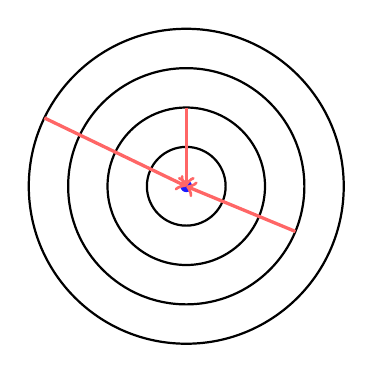
\begin{tikzpicture}


 \draw[thick](0,0) circle (0.5);
 \draw[thick](0,0) circle (1);
 \draw[thick](0,0) circle (1.5);
 \draw[thick](0,0) circle (2);
 
 
    \node at (0, 0)[circle, blue!90, fill,inner sep=1.5pt]{};
    
 \draw[->, very thick, color=red!60] (-1.8019, 0.8678) -- (0,0);

 \draw[->, very thick, color=red!60] (1.3858, -.5740) -- (0,0);

 \draw[->, very thick, color=red!60] (0, 1) -- (0,0);



\end{tikzpicture}



\begin{center}
	Ideal case $\kappa=1$
\end{center}

\end{column}

\begin{column}{.7\textwidth}


\begin{center}
	\includegraphics[width=0.7\textwidth]{bad.png}
\end{center}



\begin{center}
	When $\kappa \gg 1$
\end{center} 



\end{column}

\end{columns}


\vspace{1em}


\alert{ The method of steepest descent slows down for ill-condition matrices.}

\end{frame}



%-=-=-=-=-=-=-=-=-=-=-=-=-=-=-=-=-=-=-=-=-=-=-=-=
%	FRAME:
%-=-=-=-=-=-=-=-=-=-=-=-=-=-=-=-=-=-=-=-=-=-=-=-=
\begin{frame}{Steepest descent: FDM and FEM}
For a finite difference  5-point stencil, the matrix $A$ that we obtain has $\kappa_2(A) \sim h^{-2}$
\vspace{1em}


For FEM + nodal basis  gives matrices with $\kappa_2(A) \le C h^{-2}$

\vspace{1em}

For a uniform mesh on a square we have $\kappa_2(A) = \frac{2}{\pi^2h^2}+O(1)$


\vspace{1em}
Refine our mesh to get smaller error, $\kappa_2(A)$ grows and steepest descent slows down.

\end{frame}


%-=-=-=-=-=-=-=-=-=-=-=-=-=-=-=-=-=-=-=-=-=-=-=-=
%	FRAME:
%-=-=-=-=-=-=-=-=-=-=-=-=-=-=-=-=-=-=-=-=-=-=-=-=
\begin{frame}{Steepest descent: number of iteration}


Want 
\begin{equation*}
 \left( \frac{\kappa -1}{\kappa+1} \right)^n < \epsilon.
\end{equation*}
Where
\begin{equation*}
\frac{\kappa-1}{\kappa+1}=1-\frac{2}{\kappa+1} \sim 1- \frac{2}{\kappa}, \qquad \mbox{for large $\kappa$}.
\end{equation*}

So we have
\begin{align*}
&n\log\left(1-\frac{2}{\kappa}\right) < \log(\epsilon),\\
\implies &\frac{-2n}{\kappa} < \log(\epsilon), &&\mbox{by  Taylor approximation (as $\frac{2}{\kappa}$ is small)}\\
\implies &n > \log\left(\frac{1}{\epsilon}\right) \frac{\kappa}{2},\\
& \mbox{i.e. } n \propto \kappa_2(A).
\end{align*}



 
\end{frame}
   
   
   
   

%-=-=-=-=-=-=-=-=-=-=-=-=-=-=-=-=-=-=-=-=-=-=-=-=
%	FRAME:
%-=-=-=-=-=-=-=-=-=-=-=-=-=-=-=-=-=-=-=-=-=-=-=-=
\begin{frame}{Steepest descent: compare with sparse Cholesky factorization  }


In 2D, $\kappa_2(A) \sim h^{-2} \sim m^2$ for an $m  \times m$ grid,
so \begin{align*}
\mbox{Total work} \sim& \mbox{ \#iterations} \times \mbox{ ops/iteration}\\
=&m^2 \times 5m^2\\
=&O(m^4).
\end{align*}
which is worse asymptotically than sparse Cholesky factorisation.


\vspace{1em}


In 3D, $\kappa_2(A) \sim h^{-2}$ as well, so we use $O(m^5)$ operations to solve our system -- this is already better than sparse Cholesky. But, for the \nth{4} order biharmonic equation arising in elasticity, $\nabla^2\nabla^2u=f$, $\kappa_2(A) \sim h^{-4}$ i.e. slowdown is worse. 
 
\end{frame}



%-=-=-=-=-=-=-=-=-=-=-=-=-=-=-=-=-=-=-=-=-=-=-=-=
%	FRAME:
%-=-=-=-=-=-=-=-=-=-=-=-=-=-=-=-=-=-=-=-=-=-=-=-=
\begin{frame}{Conjugate gradient method:idea }

\alert{Idea}: Choose different directions $\vec{p}_k$, constructed from steepest descent directions $\vec{r}_k$, which have very nice properties.

 
 \vspace{0.2em}
 
 In particular, once we have searched along a particular direction, we never want to search in that direction again. 
\begin{itemize} 
	\item $\vec{x}_1$ minimises $\phi$ when searching over $\{\vec{p}_1\}$ [as before]
	\item $\vec{x}_2$ minimises $\phi$ when searching over span$\{\vec{p}_1,\vec{p}_2\}$  [not true of steepest descent]
	\item $\vec{x}_3$ minimises $\phi$ when searching over span$\{\vec{p}_1,\vec{p}_2,\vec{p}_3\}$
	 $\phantom{asdfasdfasfdasdasdsd}\vdots$
\end{itemize}






By making $x_k$ minimise $\phi$ over nested subspaces, 
we never `backtrack' or search along previous directions, so 
\[\phi(\vec{x}_{k+1}) \le \phi(\vec{x}_k),\]
i.e. $\phi$ decreases monotonically.
 
 
  \vspace{0.2em}

 
\alert{The hard part: making this cheap.}
 
\end{frame}
      
      
      
      
\begin{frame}{Conjugate gradient method: solution to hard problem}
We want to construct $\{\vec{p}_j\}$ so that
\begin{align*}
\alpha_k =\min_\alpha \phi(\vec{x}_{k-1}+\alpha \vec{p}_k)
\end{align*}
 also minimises $\phi$ over $x \in \operatorname{span}\{\vec{p}_1,\ldots,\vec{p}_k\}$.

Let's try generating $ \vec{p}_1$:
\begin{enumerate}
\item [1.]  Guess $\vec{x}_0, \vec{p}_0$ [often $\vec{x}_0=\vec{0}$, $\vec{p}_0 = \vec{r}_0 =\vec{b}$]

\end{enumerate}

\end{frame}


\begin{frame}{Conjugate gradient method: solution to hard problem}
\begin{enumerate}
\item [2.] Find $\alpha_0$ by a 1D minimisation of $\phi(\vec{x}_0+\alpha \vec{p}_0)$
\begin{align*}\vec{p}_1
\phi(\vec{x}_0 + \alpha \vec{p}_0) =& \frac{1}{2} (\vec{x}_0+\alpha \vec{p}_0)^T A (\vec{x}_0 + \alpha \vec{p}_0) - (\vec{x}_0 + \alpha \vec{p}_0)^T \vec{b}\\
=& \frac{1}{2}\vec{x}_0^T A \vec{x}_0 - \vec{x}_0^T \vec{b} + \frac{1}{2} \alpha^2 \vec{p}_0^T A \vec{p}_0 + \alpha \vec{p}_0^T A \vec{x}_0 - \alpha \vec{p}_0^T \vec{b},
\end{align*}
\begin{equation*}
\frac{d}{d \alpha}(\phi(\vec{x}_0 + \alpha \vec{p}_0) =\vec{0} \implies \alpha \vec{p}_0^T A \vec{p}_0 = \vec{p}_0^T(\vec{b}-A\vec{x}) = \vec{p}_0^T \vec{p}_0,
\end{equation*}
so that we get
\begin{align*}
\alpha_0 =& \frac{\vec{p}_0^T \vec{p}_0}{\vec{p}_0^T A \vec{p}_0},\quad
\vec{x}_1 =& \vec{x}_0 + \alpha_0 \vec{p}_0,\quad
\vec{r}_1 =& \vec{r}_0 - \alpha_0 \underbrace{A\vec{p}_0}_{\vec{w}_0},
\end{align*}
as for the first step of steepest descent% but with $\vec{p}_0$ so far unspecified. 	
\end{enumerate}
\end{frame}

\begin{frame}{Conjugate gradient method: solution to hard problem}
%\footnotesize
\begin{enumerate}
%\item  Guess $\vec{x}_0, \vec{p}_0$ [often $\vec{x}_0=\vec{0}$, $\vec{p}_0 = \vec{r}_0 =\vec{b}$]
%\item Find $\alpha_0$ by a 1D minimisation of $\phi(\vec{x}_0+\alpha \vec{p}_0)$
%\begin{align*}\vec{p}_1
%\phi(\vec{x}_0 + \alpha \vec{p}_0) =& \frac{1}{2} (\vec{x}_0+\alpha \vec{p}_0)^T A (\vec{x}_0 + \alpha \vec{p}_0) - (\vec{x}_0 + \alpha \vec{p}_0)^T \vec{b}\\
%=& \frac{1}{2}\vec{x}_0 A \vec{x}_0 - \vec{x}_0^T \vec{b} + \frac{1}{2} \alpha^2 \vec{p}_0^T A \vec{p}_0 + \alpha \vec{p}_0^T A \vec{x}_0 - \alpha \vec{p}_0^T \vec{b},
%\end{align*}
%\begin{equation*}
%\frac{d}{d \alpha}(\phi(\vec{x}_0 + \alpha \vec{p}_0) =\vec{0} \implies \alpha \vec{p}_0^T A \vec{p}_0 = \vec{p}_0^T(\vec{b}-A\vec{x}) = \vec{p}_0^T \vec{p}_0,
%\end{equation*}
%so that we get
%\begin{align*}
%\alpha_0 =& \frac{\vec{p}_0^T \vec{p}_0}{\vec{p}_0^T A \vec{p}_0},\quad
%\vec{x}_1 =& \vec{x}_0 + \alpha_0 \vec{p}_0,\quad
%\vec{r}_1 =& \vec{r}_0 - \alpha_0 \underbrace{A\vec{p}_0}_{\vec{w}_0},
%\end{align*}
%as for the first step of steepest descent% but with $\vec{p}_0$ so far unspecified. 
\item [3.] Find $\vec{x}_2$ by 2D minimisation of
\begin{align*}
\phi(\vec{x}_0 + \alpha_0 \vec{p}_0 + \alpha_1 \vec{p}_1) =& \phi(\vec{x}_1 + \alpha_1 \vec{p}_1)\\
=&\frac{1}{2}(\vec{x}_1 + \alpha_1 \vec{p}_1)^T A (\vec{x}_1 + \alpha_1 \vec{p}_1) - (\vec{x}_1 + \alpha_1 \vec{p}_1)^T \vec{b}\\
=& \underbrace{\frac{1}{2}\vec{x}_1^TA\vec{x}_1 - \vec{x}_1^T\vec{b}}_{\phi(\vec{x}_1)} + \frac{1}{2} \alpha_1^2 \vec{p}_1^T A \vec{p}_1 + \underbrace{\alpha_1 \vec{p}_1^T A \vec{x}_1 - \alpha_1 \vec{p}_1^T \vec{b}}_{-\alpha_1 \vec{p}_1^T\vec{r}_1}\\
=&\phi(\vec{x}_1) + \frac{1}{2} \alpha_1^2 \vec{p}_1^T A \vec{p}_1 - \alpha_1 \vec{p}_1^T(\vec{r}_0 - \alpha_0 A \vec{p}_0),
\end{align*}
where we note that $\beta\alpha \vec{p}_1^TA\vec{p}_0$ is the only term that includes $\alpha_1$ and $\alpha_0$. 
We can de-couple the 2D minimisation of $\phi$ into two 1D minimizations if we set  this term to zero by choosing
\[\vec{p}_1^TA\vec{p}_0=0.\] 
\end{enumerate}


\alert{Note}: Local minimisation also gives us the global minimum. 

\end{frame}













\begin{frame}{Conjugate gradient method: conjugate direction}
Two vectors that satisfy $\vec{u}^{\rm T}A \vec{v}=0$ are called \emph{$A$-conjugate}.




\vspace{1em}

If $A$ is symmetric we can define an inner product $( \vec{u},\vec{v} )_A \equiv \vec{u}^T A\vec{v}$.
If $A$ is also positive definite, this induces a norm $\|\vec{u}\|^2_A \equiv <\vec{u}, \vec{u}>_A= \vec{u}^T A\vec{u}$. So A-conjugate vectors are orthogonal wrt the 
A-inner product. 

\vspace{1em}


Aim to produce a set of mutually A-conjugate vectors. To achieve this we do conjugate Gram-Schmidt to form $\{\vec{p}_0,\vec{p}_1,\ldots\}$, from $\{\vec{r}_0,\vec{r}_1,\ldots\}$.

\end{frame}


      

%-=-=-=-=-=-=-=-=-=-=-=-=-=-=-=-=-=-=-=-=-=-=-=-=
%	FRAME:
%-=-=-=-=-=-=-=-=-=-=-=-=-=-=-=-=-=-=-=-=-=-=-=-=
\begin{frame}{Conjugate gradient method: algorithm}

\begin{enumerate}
\item [1.] Guess $\vec{p}_0=\vec{r}_0$.
\item [2.] Let \begin{align*}
\alpha_0 = & \frac{\vec{r}_0^T\vec{r}_0}{\vec{p}_0^TA\vec{p}_0},\quad
\vec{x}_1 = & \vec{x}_0+\alpha_0\vec{p}_0,\quad 
\vec{r}_1 = & \vec{r}_0-\alpha_0A\vec{p}_0,
\end{align*}
as before. 
\item [3.] $\vec{p}_1 =  \vec{r}_1 - \text{component of }\vec{r}_1 \text{ not }A-\text{conjugate to }\vec{p}_0, \text{ i.e. } \vec{p}_1=  \vec{r}_1 + \beta_0 \vec{p}_0 $ (since span $\{\vec{r}_0,\vec{r}_1\}=$span $\{\vec{p}_0,\vec{p}_1\}$)
Determine $\beta_0$ by enforcing $A$-conjugacy
\begin{align*}
&\vec{p}_1^T A \vec{p}_0 = 0 \implies (\vec{r}_1 + \beta_0\vec{p}_0)^T A \vec{p}_0=0,
\implies& \beta_0=\frac{-\vec{r}_1^TA\vec{p}_0}{\vec{p}_0^TA\vec{p}_0}.
\end{align*}
Then since
\begin{equation*}
\vec{r}_1=\vec{r}_0-\alpha_0 A \vec{p}_0, \qquad -A\vec{p}_0=\frac{\vec{r}_1-\vec{r}_0}{\alpha_0},
\end{equation*}
\begin{align*}
\beta_0=\frac{\vec{r}_1^T (\vec{r}_1-\vec{r}_0)/\alpha_0}{\vec{p}_0^T A\vec{p}_0}
= \frac{\vec{r}_1^T \vec{r}_1}{\alpha_0 \vec{p}_0^T A \vec{p}_0}
=\frac{\vec{r}_1^T \vec{r}_1}{\vec{r}_0^T \vec{r}_0}, \\
(=\mbox{reduction in the square residual.})
\end{align*}

%\item So given $\vec{p}_1$, $\vec{x}_1$, $\vec{r}_1$, we calculate $\vec{p}_2$:
%\begin{align*}
%\alpha_1 = \frac{\vec{r}_1^T\vec{r}_1}{\vec{p}_1^T A \vec{p}_1}, \qquad x_2=\vec{x}_1+\alpha_1 \vec{p}_1, \qquad \vec{r}_2= \vec{r}_1-\alpha_1 A \vec{p}_1,\\\
%\beta_1=\frac{\vec{r}_2^T\vec{r}_2}{\vec{r}_1^T\vec{r}_1}, \qquad \vec{p}_2=\vec{r}_2+\beta_1 \vec{p}_1.
%\end{align*}
%
%This all leaves $\vec{r}_2 \perp \vec{r}_0, \vec{r}_1$; $\vec{p}_2$  conjugate to $\vec{p}_0, \vec{p}_1$; and  $\vec{r}_2 \perp \vec{p}_0, \vec{p}_1$ (but not $\vec{p}_2$.

\end{enumerate}


 
\end{frame}


%-=-=-=-=-=-=-=-=-=-=-=-=-=-=-=-=-=-=-=-=-=-=-=-=
%	FRAME:
%-=-=-=-=-=-=-=-=-=-=-=-=-=-=-=-=-=-=-=-=-=-=-=-=
\begin{frame}{Conjugate gradient method: algorithm}

\begin{enumerate}
%\item Guess $\vec{p}_0=\vec{r}_0$.
%\item Let \begin{align*}
%\alpha_0 = & \frac{\vec{r}_0^T\vec{r}_0}{\vec{p}_0^TA\vec{p}_0},\quad
%\vec{x}_1 = & \vec{x}_0+\alpha_0\vec{p}_0,\quad 
%\vec{r}_1 = & \vec{r}_0-\alpha_0A\vec{p}_0,
%\end{align*}
%as before. 
%\item  $\vec{p}_1 =  \vec{r}_1 - \text{component of }\vec{r}_1 \text{ not }A-\text{conjugate to }\vec{p}_0 =  \vec{r}_1 + \beta_0 \vec{p}_0 \qquad $ (since span $\{\vec{r}_0,\vec{r}_1\}=$span $\{\vec{p}_0,\vec{p}_1\}$)
%Determine $\beta_0$ by enforcing $A$-conjugacy
%\begin{align*}
%&\vec{p}_1^T A \vec{p}_0 = 0 \implies (\vec{r}_1 + \beta_0\vec{p}_0)^T A \vec{p}_0=0,
%\implies& \beta_0=\frac{-\vec{r}_1^TA\vec{p}_0}{\vec{p}_0^TA\vec{p}_0}.
%\end{align*}
%Then since
%\begin{equation*}
%\vec{r}_1=\vec{r}_0-\alpha_0 A \vec{p}_0, \qquad -A\vec{p}_0=\frac{\vec{r}_1-\vec{r}_0}{\alpha_0},
%\end{equation*}
%\begin{align*}
%\beta_0=\frac{\vec{r}_1^T (\vec{r}_1-\vec{r}_0)/\alpha_0}{\vec{p}_0^T A\vec{p}_0}
%= \frac{\vec{r}_1^T \vec{r}_1}{\alpha_0 \vec{p}_0^T A \vec{p}_0}
%=\frac{\vec{r}_1^T \vec{r}_1}{\vec{r}_0^T \vec{r}_0}, \\
%(=\mbox{reduction in the square residual.})
%\end{align*}

\item [4.] So given $\vec{p}_1$, $\vec{x}_1$, $\vec{r}_1$, we calculate $\vec{p}_2$:
\begin{align*}
\alpha_1 = \frac{\vec{r}_1^T\vec{r}_1}{\vec{p}_1^T A \vec{p}_1}, \qquad x_2=\vec{x}_1+\alpha_1 \vec{p}_1, \qquad \vec{r}_2= \vec{r}_1-\alpha_1 A \vec{p}_1,\\\
\beta_1=\frac{\vec{r}_2^T\vec{r}_2}{\vec{r}_1^T\vec{r}_1}, \qquad \vec{p}_2=\vec{r}_2+\beta_1 \vec{p}_1.
\end{align*}

This all leaves $\vec{r}_2 \perp \vec{r}_0, \vec{r}_1$; $\vec{p}_2$  conjugate to $\vec{p}_0, \vec{p}_1$; and  $\vec{r}_2 \perp \vec{p}_0, \vec{p}_1$ (but not $\vec{p}_2$.

\end{enumerate}

After $k$ iterations, 
\begin{align*}
\vec{x}_k= \mbox{solution that minimizes $\phi$ over $x \in \vec{x}_0+\mbox{span}\{\vec{p}_0,\vec{p}_1,\ldots,\vec{p}_{k-1}\}$}
\end{align*}


 
\end{frame}





%-=-=-=-=-=-=-=-=-=-=-=-=-=-=-=-=-=-=-=-=-=-=-=-=
%	FRAME:
%-=-=-=-=-=-=-=-=-=-=-=-=-=-=-=-=-=-=-=-=-=-=-=-=
\begin{frame}{Conjugate gradient method: property}

Minimising $\phi$ is same as minimising the error in the $A$-norm:\\$\|\vec{e}\|_A=\|\vec{x} -\vec{x}^*\|_A$.


\alert{Proof}:
\begin{align*}
\|\vec{e}\|^2_A =& \|\vec{x}-\vec{x}^*\|_A^2 = (\vec{x}-\vec{x}^*)^TA(\vec{x}-\vec{x}^*)\\
=& \vec{x}^TA\vec{x} - 2\vec{x}^TA\vec{x}^*+\vec{x}^{*T}A\vec{x}^*\\
=& \underbrace{\vec{x}^TA\vec{x} - 2\vec{x}^T\vec{b}}_{2\phi(\vec{x})} + \underbrace{\vec{x}^{*T}A\vec{x}^*}_{\mbox{constant}}
\end{align*}


$\vec{x}_k$ minimises $\|\vec{e}\|_A$ over $\vec{x}_0 + \mbox{span}\{\vec{p}_0, \ldots, \vec{p}_{k-1}\}$. But

\begin{equation*}
\vec{r}_0=\vec{p}_0,\vec{r}_1=\vec{r}_0-\alpha_0 A \vec{p}_0,\vec{r}_2=\vec{r}_1 - \alpha_1 A\vec{p}_1. \ldots
\end{equation*}
so
\begin{equation*}
\mbox{span}\{\vec{p}_0,\vec{p}_1,\ldots,\vec{p}_{k-1}\} = \underset{\mbox{\alert{Krylov Space}}}{\mbox{span} \{\vec{r}_0, A\vec{r}_0, A^2\vec{r}_0,\ldots,A^{k-1}\vec{r}_0\}}.
\end{equation*}
 
\end{frame}






%-=-=-=-=-=-=-=-=-=-=-=-=-=-=-=-=-=-=-=-=-=-=-=-=
%	FRAME:
%-=-=-=-=-=-=-=-=-=-=-=-=-=-=-=-=-=-=-=-=-=-=-=-=
\begin{frame}{Conjugate gradient method: property}
Since $A\vec{x}=\vec{b}-\vec{r}$ and $A\vec{x}^*=\vec{b}$, $A\vec{e}=-\vec{r}$, so
\begin{align*}
\mbox{span}\{\vec{p}_0,\vec{p}_1,\ldots,\vec{p}_{k-1}\} =& \mbox{span} \{\vec{r}_0, A\vec{r}_0, A^2\vec{r}_0,\ldots,A^{k-1}\vec{r}_0\}\\ =& \mbox{span}\{A\vec{e}_0,A^2\vec{e}_0,\ldots,A^k\vec{e}_0\}
\end{align*}
so 
\begin{equation*}
\vec{x}_k = \vec{x}_0 + \mbox{Linear combinations}\{A\vec{e}_0,\ldots,A^k\vec{e}_0\}
\end{equation*}

If we subtract $\vec{x}^*$ from both sides then
\begin{equation*}
\vec{e}_k=\vec{e}_0+\mbox{Linear combinations}\{A\vec{e}_0,\ldots,A^k\vec{e}_0\} = P_k(A)\vec{e}_0
\end{equation*}
where $P_k$ is a polynomial of degree k with $p(0)=1$.

Since conjugate-gradient minimises $\phi(x)$ and $\|\vec{e}\|_A$ over $\mathcal{K}_k$, 
\begin{equation*}
\|\vec{e}_k\|_A = \min_{p \in P_k} \|p(A)\vec{e}_0\|_A.
\end{equation*}

$\Rightarrow$ \alert{ Conjugate gradient converges to the exact answer in $N$ iterations (ignoring roundoff).}
 
\end{frame}







%-=-=-=-=-=-=-=-=-=-=-=-=-=-=-=-=-=-=-=-=-=-=-=-=
%	FRAME:
%-=-=-=-=-=-=-=-=-=-=-=-=-=-=-=-=-=-=-=-=-=-=-=-=
\begin{frame}{Conjugate gradient method: example}
If $A$ has only $k <N$ different eigenvalues  then conjugate gradient converges in $k$ iterations.


\alert{Proof}
The polynomial of degree $k$:
\begin{equation*}
\prod_{i=1}^k \left(1- \frac{x}{\lambda_i}\right),
\end{equation*}
has $p(0)=1$, but $p(\lambda_i)=0 \implies \vec{e}_k=\vec{0}.$




\vspace{1em}

If we don't know the spectrum of $A$ but only know $\lambda \in (\lambda_{\min},\lambda_{\max})$, then the best result is:
\begin{equation}\label{CGcgce}
\frac{\|\vec{e}_k\|_A}{\|\vec{e}_0\|} \le 2 \left( \frac{\sqrt{\kappa}-1}{\sqrt{\kappa}+1} \right)^k,
\end{equation}
where $\kappa = \kappa_2(A) = \frac{\lambda_{\max}}{\lambda_{\min}}$.

So if $\kappa$ is near 1, i.e. $\lambda_{\max} - \lambda_{\min} \ll \lambda_{\max} + \lambda_{\min}$, then convergence is rapid.

 
\end{frame}



%-=-=-=-=-=-=-=-=-=-=-=-=-=-=-=-=-=-=-=-=-=-=-=-=
%	FRAME:
%-=-=-=-=-=-=-=-=-=-=-=-=-=-=-=-=-=-=-=-=-=-=-=-=
\begin{frame}{Conjugate gradient method: number of iteration}
 
 
 
Estimate a (pessimistic) bound for the number of iterations to achieve a tolerance $\epsilon$:
\[n > \frac{\sqrt{\kappa}}{2} \log\left(\frac{2}{\epsilon}\right).\]
So we need $\sim \sqrt{\kappa}$ iterations for CG to achieve convergence. 

\vspace{0.6em}

For a 5-point FD stencil or $P_1$ or $Q_1$ FEM, $\kappa_2 \sim h^{-2} \sim m^2$.
So if we require $\sim\sqrt{\kappa_2}$ iterations then the total work is $O(m^3)$ to find the solution -- the same complexity as \textbackslash $\,$ in 2D.




\vspace{0.6em}

In 3D we have $\sim m$ iterations at $O(m^3)$ operations per iteration, so $O(m^4)$, compared to $O(m^6)$ for \textbackslash.

 
\end{frame}





%-=-=-=-=-=-=-=-=-=-=-=-=-=-=-=-=-=-=-=-=-=-=-=-=
%	FRAME:
%-=-=-=-=-=-=-=-=-=-=-=-=-=-=-=-=-=-=-=-=-=-=-=-=
\begin{frame}{Conjugate gradient method: Numerical example}
 
 \begin{center}
 	  \includegraphics[width=0.65\textwidth]{CG_test.pdf}
 \end{center}
 

CG converges faster if the spectrum is `nice', we look for ways to improve the spectrum, i.e. \alert{preconditioning}.
 
\end{frame}



%-=-=-=-=-=-=-=-=-=-=-=-=-=-=-=-=-=-=-=-=-=-=-=-=
%	FRAME:
%-=-=-=-=-=-=-=-=-=-=-=-=-=-=-=-=-=-=-=-=-=-=-=-=
\begin{frame}{Preconditioned conjugate gradient (PCG): idea}
Instead of solving $A\vec{x}=\vec{b}$, solve $M^{-1}A\vec{x}=M^{-1}\vec{b}$ such that:
\begin{itemize}
\item  it must be cheap to solve $M\vec{z}=\vec{r}$ (which is the only place $M$ enters in the PCG algorithm)
\item $M^{-1}A$ must be sparse and symmetric positive definite (if $A$ is)
\item $M^{-1}A$ has a `nicer' spectrum, e.g.\ $\kappa_2(M^{-1}A) \ll \kappa_2(A)$
\end{itemize}

\vspace{0.5em}

Choice of $M$:
\begin{itemize}
	\item If $M=I$ then $M\vec{z}=\vec{r}$ is easy to solve, but $\Lambda(M^{-1}A) = \Lambda(A)$ and we haven't done anything.
	\item If $M=A$ now $\Lambda(M^{-1}A) = \Lambda(I)$ which is perfect but $M\vec{z}=\vec{r}$ is $A\vec{z}=\vec{r}$ which is just our original problem.
\end{itemize}




look for $M$ that `approximates' $A$ so that the eigenvalues of $M^{-1}A$ are more clustered than $A$.
We often look for a factorised $M=M_1M_2$ where $M_1$, $M_2$ are cheap to invert, e.g.\ Cholesky factors $M = L L^T = R^T R$
 
\end{frame}

	



%-=-=-=-=-=-=-=-=-=-=-=-=-=-=-=-=-=-=-=-=-=-=-=-=
%	FRAME:
%-=-=-=-=-=-=-=-=-=-=-=-=-=-=-=-=-=-=-=-=-=-=-=-=
\begin{frame}{PCG: choice of preconditioner}
	
	
	\alert{There are \emph{no} magical preconditioners!}

The best comes from a deep knowledge of $A$ and where it came from.
They  often come from approximating $A$ or solving a related simpler problem cheaply to get an approximation.

Some candidates that are symmetric positive definite and sparse:
\begin{itemize}
\item Jacobi (point), $M_J = D = \operatorname{diag}(A)$.

This has modest benefit unless the diagonal elements of $A$ vary greatly.  It has no effect on $A_5$ (since the diagonal elements are all the same).

\item Incomplete factorisations

For these we go through the process of (Cholesky) factorisation but prevent or reduce the amount of fill-in.
So the matrix obtained is sparser than usual sparse Cholesky factorisation (less fill-in) but only gives an approximate factorisation.
\end{itemize}
	
\end{frame}



%-=-=-=-=-=-=-=-=-=-=-=-=-=-=-=-=-=-=-=-=-=-=-=-=
%	FRAME:
%-=-=-=-=-=-=-=-=-=-=-=-=-=-=-=-=-=-=-=-=-=-=-=-=
\begin{frame}{PCG: incomplete Cholesky factorisation}
	
	
	Direct Cholesky (\textbackslash)
\begin{equation*}
A=R^TR \mbox{ or } L L^T.
\end{equation*}

Incomplete Cholesky
\begin{equation*}
A= \bar{R}^T \bar{R} + \underbrace{\epsilon}_{\mbox{error}},
\end{equation*}
where $\bar{R}^T\bar{R}=M$ is  a preconditioner, $M=M_1M_2=\bar{R}^T\bar{R}$ ( or $M = \bar{L}\bar{L}^T$).


Matlab has (as at 2012):
\begin{itemize}
\item Incomplete Cholesky with no fill-in 

$L = ichol(A)$, which you then use in a call to $pcg$:

$[  ,   ,   ,  ] = pcg(A,b,tol,maxits, L, L')$

This only allows non-zeroes of $L$ where $A$ has non-zeroes i.e. no fill-in.
To call CG in {\sc{Matlab}}, use $pcg$ with no preconditioner:

$[  ,   ,   ,  ] = pcg(A,b,tol,maxits)$



\end{itemize}

	
\end{frame}




%-=-=-=-=-=-=-=-=-=-=-=-=-=-=-=-=-=-=-=-=-=-=-=-=
%	FRAME:
%-=-=-=-=-=-=-=-=-=-=-=-=-=-=-=-=-=-=-=-=-=-=-=-=
\begin{frame}{PCG: incomplete Cholesky factorisation}
	
	

\begin{itemize}

\item Modified incomplete Cholesky

Where the matrix $A$ has come from an elliptic PDE (as in our cases), it is better when you delete an entry that would  have produced fill-in 
to add that entry to the diagonal entry on the same row, so that $A\vec{x} = \bar{L}\bar{L}^T\vec{x}$ when $\vec{x}$ is a constant vector. This is called 
Modified incomplete Cholesky (MIC) factorization. This can be called in {\sc{Matlab}} by accessing the $options$ structure in the call to $ichol$:

$options.type = 'nofill';$\\
$options.michol = 'on';$\\
$L = ichol(A,options)$

Supposedly, for $A_5$ this can reduce $\kappa_2(M^{-1}A)$ to $O(h^{-1})$.

With this preconditioner,  PCG has $\sqrt{\kappa} \sim m^{\frac{1}{2}}$ iterations, so the total work is $O(m^{2.5})$ in 2D, $O(m^{3.5})$ in 3D.
This is called \emph{optimal PCG} (for $A_5$) .


\end{itemize}

	
\end{frame}





%-=-=-=-=-=-=-=-=-=-=-=-=-=-=-=-=-=-=-=-=-=-=-=-=
%	FRAME:
%-=-=-=-=-=-=-=-=-=-=-=-=-=-=-=-=-=-=-=-=-=-=-=-=
\begin{frame}{PCG: incomplete Cholesky factorisation}
	
	

\begin{itemize}


\item Incomplete Cholesky with a drop tolerance

$options.type = 'ict';$\\
$options.droptol = 0.05;$\\
$L = ichol(A,options)$

This throws away the fill-in entries smaller  than a certain size determined by the drop tolerance. 
For large drop tolerance, this is the same as the no-fillin case (the default); 
% as $\mbox{drop tolerance} \to 0$, $L \to \mbox{same Cholesky factor as produced by  \textbackslash}$ (same fill-in as \textbackslash).


\end{itemize}

	
\end{frame}




%-=-=-=-=-=-=-=-=-=-=-=-=-=-=-=-=-=-=-=-=-=-=-=-=
%	FRAME:
%-=-=-=-=-=-=-=-=-=-=-=-=-=-=-=-=-=-=-=-=-=-=-=-=
\begin{frame}{PCG: Numerical example}
 
 \begin{center}
 	  \includegraphics[width=0.65\textwidth]{it_solve128.pdf}
 \end{center}

 
\end{frame}


%-=-=-=-=-=-=-=-=-=-=-=-=-=-=-=-=-=-=-=-=-=-=-=-=
%	FRAME:
%-=-=-=-=-=-=-=-=-=-=-=-=-=-=-=-=-=-=-=-=-=-=-=-=
\begin{frame}[standout]
  End of week 7!
\end{frame}

\appendix



\end{document}
